\documentclass{article}
\usepackage[utf8]{inputenc}
\usepackage[spanish]{babel}
\usepackage{graphicx}
\usepackage{color}
\graphicspath{ {c:/user/images/} }

\begin{document}
\begin{center}

\includegraphics[scale=0.12]{escudo.png}
\end{center}
\vspace{50pt}
\begin{center}
\bf{\sc\Large 'Interrupciones en el microprocesador'}\\
\end{center}
\vspace{50pt}
\begin{center}
\begin{center}
\bf{\sc\large Por:}\\
\end{center}
\bf{\sc\large María Salomé Garcés Montero}\\
\end{center}
\vspace{60pt}
\begin{center}
\bf{\sc\large Facultad de ingeniería}\\
\end{center}
\begin{center}
\bf{\sc\large Medellín}
\end{center}
\begin{center}
\bf{\sc\large 2020}\\
\end{center}\
\newpage
\begin{center}
\bf{\sc\LARGE Interrupciones en el microprocesador}\\
\end{center}
\vspace{50pt}
\large 
Se puede decir que el microprocesador es el dispositivo más importante en un computador, pues encargado de ejecutar los programas, instrucciones y tareas en este. Otra de sus funciones principales es como su nombre lo indica, procesar los datos que ingresan y salen del dispositivo.

\vspace{10pt}
En los primeros sistemas de cómputo se realizaba un muestreo constante del hardware de entrada o salida en los periféricos del computador para determinar si estos enviaban algún dato que necesitase ser atendido por el procesador; esta tarea se conoce como técnica de sondeo. 
El problema con esta técnica es su poca eficiencia, pues el estar muestreando periódicamente los puertos de entrada implica un alto consumo de recursos.
Como solución a esto se implementaron las llamada interrupciones, en las cuales el dispositivo externo es el encargado de indicarle al procesador que debe ser atendido. Esta indicación frena la ejecución de otros programas y prioriza los datos del dispositivo o programa que la envía. Cuando se termina la acción solicitada por la interrupción la central de procesamiento continúa con la tarea que venía realizando. De esta forma se evita que se esté en constante verificación y se previene el uso innecesaria de recursos. 

\vspace{10pt}
Existen dos tipos principales de interrupciones: la interrupción por hardware y la interrupción por software. La primera se da como respuesta a un dispositivo que se conecta a uno de los periféricos del computador. Este envía una señal a la unidad central de procesamiento para que se realicen las operaciones correspondientes. Por otro lado las interrupciones de software suceden cuando el usuario envía la indicación al sistema para que se detenga la tarea que se está ejecutando y se realice una diferente; otro caso posible para que se de una interrupción por software es cuando se notifica un error en algún programa y es necesario que este se suspenda. La eficiencia en ambos tipos de interrupcion tiene relación directa con el lenguaje de programación y el tipo de hardware utilizados, pues de estos dependerá en parte la velocidad del procesamiento de los datos.
\newpage
En la Ilustración 1 se muestra una interrupción implementada en una placa de arduino: 
\vspace{10pt}
\begin{center}
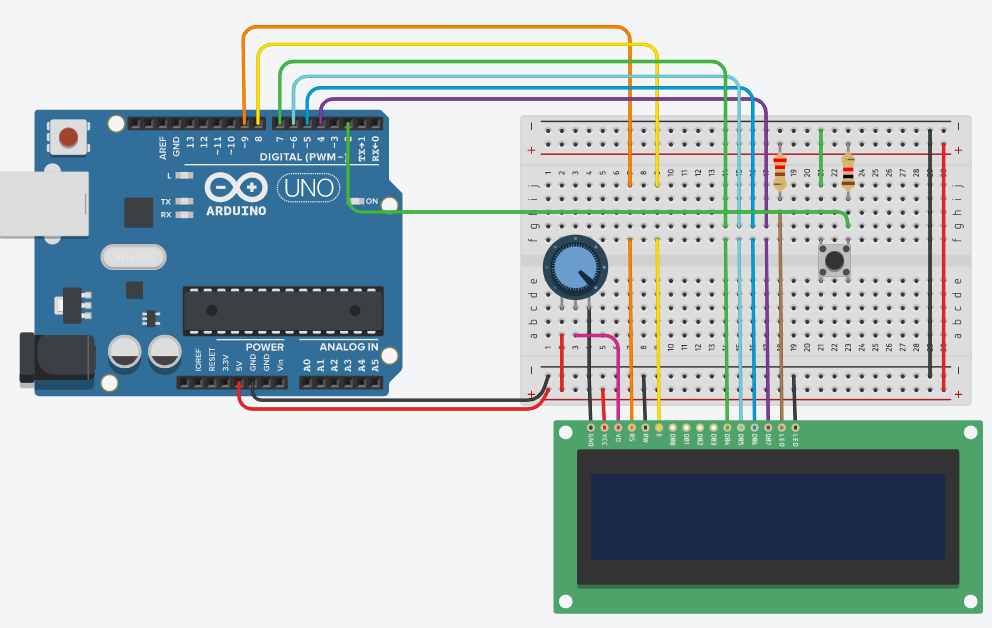
\includegraphics[scale=0.6]{arduino.png}
\normalsize
Ilustración 1. Simulación en tinkercad.
\end{center}
\vspace{20pt}
\large
Su funcionamiento es muy simple: la LCD opera a modo de contador, en ella se muestran números de 1 a 60, cambiando cada segundo. Cuando se presiona el pulsador se ejecuta la interrupción y se empieza a realizar la tarea correspondiente a dicha instrucción, que consiste en mostrar en la LCD los días de la semana en un intervalo de dos segundos entre cada uno.La interrupción se implenta usando la función attachInterrupt(),en la cual se indica el pin o puerto en que se dará la indicación,la acción a realizar y el modo del pin.
\vspace{10pt}

Una vez terminada la tarea de imprimir los días, se retoma la operación de conteo de números.

\newpage
Código de arduino:
\vspace{10pt}
\begin{center}
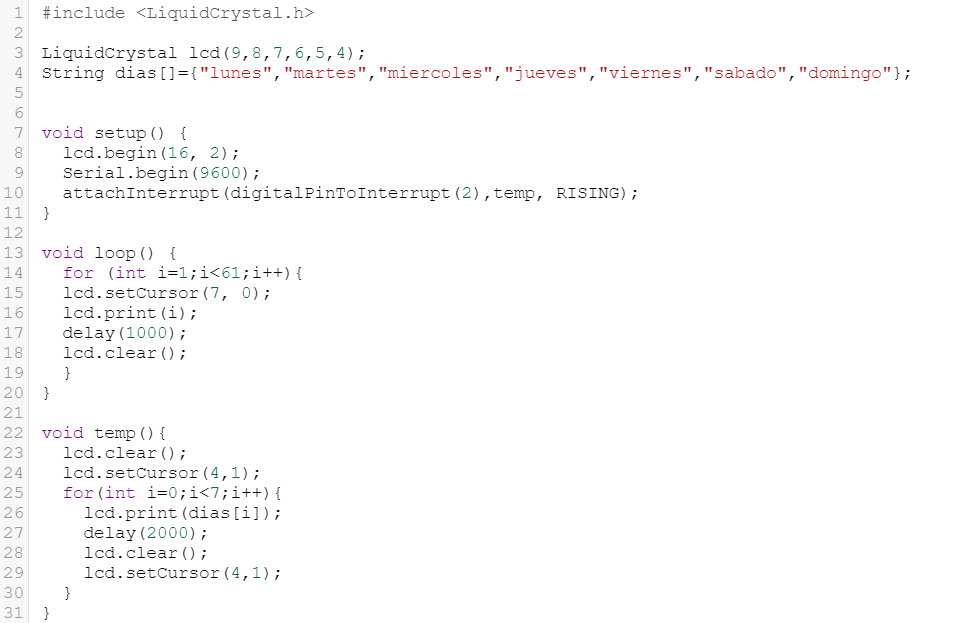
\includegraphics[scale=0.8]{código.png}
\end{center}
\newpage
\begin{thebibliography}{0}

\bibitem{NN2003} Niño,J. (2003). Las interrupciones.
Recuperado de 
 \href{\textcolor{blue}{http://www.angelfire.com/al4/pc/int.htm}}
   
 \bibitem{2019} (2019). Interrupciones y excepciones. Sistemas operativos -Universidad de Sevilla.

Recuperado de 
   \href{\textcolor{blue}{https://1984.lsi.us.es/wiki-ssoo/index.php/Interrupciones_y_excepciones}}
   
\bibitem{Casta} Castaño,S. Interrupciones con arduino.Control autmático educación.

 Recuperado de 
 \href{\textcolor{blue}{https://controlautomaticoeducacion.com/arduino/interrupciones-arduino/}} 

 \bibitem{NN} Interrupciones hardware. La web se sistemas operativos.

 Recuperado de 
   \href{\textcolor{blue}{http://sopa.dis.ulpgc.es/ii-dso/leclinux/interrupciones/int_hard/LEC3_INT_HARD.pdf}}

 \bibitem{NN} Arquitectura de Computadoras – Interrupciones.

 Recuperado de 
   \href{\textcolor{blue}{https://www.fing.edu.uy/tecnoinf/mvd/cursos/arqcomp/material/teo/arq-teo08.pdf}}
   
\end{thebibliography}
\end{document}